%!TEX options = -shell-escape

\documentclass[glossy]{beamer}

% Fonts
\usepackage[utf8]{inputenc}
\usepackage{lmodern}
\usepackage[T1]{fontenc}

% Beamer
\useoutertheme{wuerzburg}
\useinnertheme[realshadow,corners=2pt,padding=2pt]{chamfered}
\usecolortheme{shark}

\setbeamertemplate{navigation symbols}{}

% Tikz
\usepackage{tikz}
\usetikzlibrary{tikzmark, arrows, decorations, decorations.pathreplacing}
\tikzset{every picture/.style={font issue=\scriptsize},
         font issue/.style={execute at begin picture={#1\selectfont}}
}

\tikzstyle{callout}=[remember picture, ->, >=stealth, overlay, red, ultra thick, align=left]

% Minted
\usepackage{minted}
\newminted{cpp}{autogobble, fontsize=\tiny, escapeinside=@@}
\newmintedfile{cpp}{autogobble, fontsize=\tiny, escapeinside=@@}
\newmintinline{cpp}{escapeinside=@@}
\newmintinline{java}{}
\newmintinline{js}{}
\usemintedstyle{vs}

% GraphicX
\usepackage{graphicx}
\graphicspath{{img/}}

% Macros
\newcommand{\cppref}[2]{\href{http://en.cppreference.com/w/cpp/#1}{\underline{#2}}}
\newcommand{\refer}[1]{([shift={(.25em,.25em)}]pic cs:#1)}

% Meta
\title{C++ Boot Camp 1/2}
\author{Jesse Talavera-Greenberg}
\date{}

\begin{document}

\begin{frame}[fragile=singleslide]
  \frametitle{C++ Boot Camp 1/2}
  \framesubtitle{Jesse Talavera-Greenberg}
  \begin{figure}
    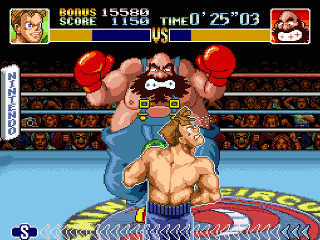
\includegraphics[width=.75\columnwidth]{super-punch-out}
    \centering
  \end{figure}
  \begin{tikzpicture}[callout, line width=2mm]
    \draw (3.5cm, 2cm) node [anchor=east] {\shortstack{\huge \textbf{You}}} -> (6.25cm, 3.5cm);
    \draw (8.5cm, 5.75cm) node [anchor=west] {\shortstack{\huge \textbf{C++}}} -> (6.5cm, 5.5cm);
  \end{tikzpicture}
\end{frame}

\begin{frame}[fragile=singleslide]
  \frametitle{Disclaimers}
  \begin{itemize}
    \item I am not the grader for this course.
    \item This boot camp is entirely voluntary.
    \item Any opinions expressed are my own.
    \item I don't know much about DirectX.
    \item Correctness is likely, but \textbf{not guaranteed}.
  \end{itemize}
\end{frame}

\begin{frame}[fragile=singleslide]
  \frametitle{This Week}
  \begin{itemize}
    \item C++ language and standard library
    \item Common traps
    \item Important concepts
    \item Go to \href{www.cppreference.com}{www.cppreference.com} to follow code in-browser
  \end{itemize}
\end{frame}

\begin{frame}[fragile=singleslide]
  \frametitle{The Big Picture}
  \begin{columns}
    \begin{column}{6cm}
      \begin{itemize}
        \item Mix high-level syntax with low-level management
        \item Originally designed for C compatibility
        \item Not your daddy's C++
      \end{itemize}
    \end{column}

    \begin{column}{6cm}
      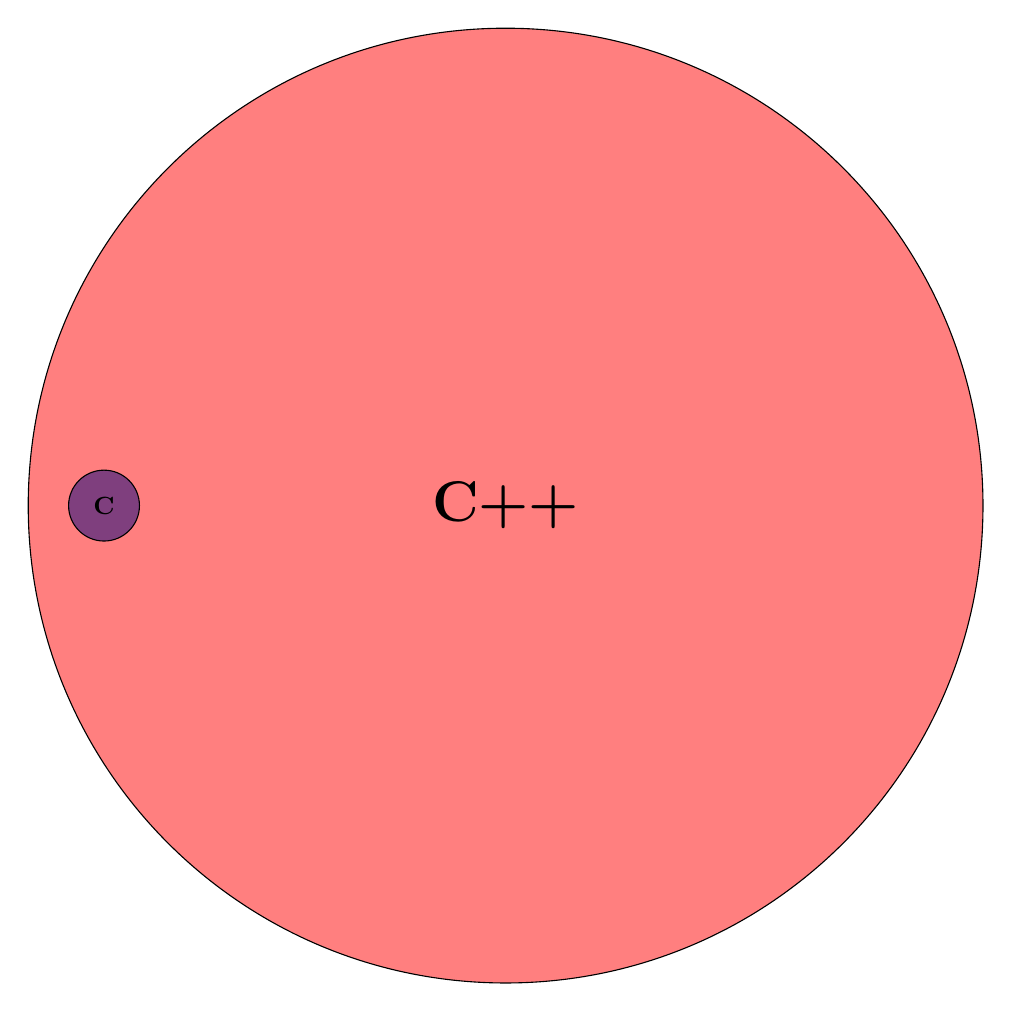
\begin{tikzpicture}[align=center, blend mode=multiply, anchor=center]
        \draw [fill=red, fill opacity=0.5] (0.4\columnwidth,8) circle (0.5\columnwidth) node [fill opacity=1] {\huge{\textbf{C++}}};
        \draw [fill=blue, fill opacity=0.5] (-0.25,8) circle (.45cm) node [fill opacity=1] {\small{\textbf{C}}};
      \end{tikzpicture}
    \end{column}
  \end{columns}
\end{frame}

\begin{frame}[fragile=singleslide]
  \frametitle{\cppref{language/basic_concepts}{The Basics}}
  \cppfile{src/basic.cpp}
  
  
\begin{tikzpicture}[callout]
    \draw (4.5cm, 26em) node [anchor=west] {\shortstack{\cppref{preprocessor/include}{Include libraries, functions, etc.}}} -> \refer{basic_include};
    \draw (7cm, 24em) node [anchor=west] {\shortstack{\# of command-line arguments}} -> \refer{basic_argc};
    \draw (7cm, 21em) node [anchor=west] {\shortstack{actual arguments as\\a string array}} -> \refer{basic_argv};
    \draw[decorate, decoration={brace}, -] ({pic cs:basic_using_a} |- {pic cs:basic_using_b}) +(0,1.5em) -- node [right, inner sep=1em] {Pulls into namespace\\(avoid long-ass prefixes)} ({pic cs:basic_using_a} |- {pic cs:basic_using_b});
    \draw (7cm, 15em) node [anchor=west] {\shortstack{\cppref{io}{Formatted printout}}} -> \refer{basic_print};
    \draw (5cm, 3em) node [anchor=west] {\shortstack{Return code (absence in main implies 0)}} -> \refer{basic_return};
    \draw (4cm, 12em) node [anchor=west] {\shortstack{Strings not allowed\\in switch statements}} -> \refer{basic_switch};
  \end{tikzpicture}
\end{frame}

\begin{frame}[fragile=singleslide]
  \frametitle{\cppref{language/types}{Fundamental Types}}
  \begin{columns}[t]
    \begin{column}{6cm}
      \begin{itemize}
        \item Integer sizes \cppref{language/types\#Data_models}{\textbf{can vary}} by platform, compiler, and OS
        \item No \javainline|byte| (use \cppinline|uint8_t|)
        \item \javainline|boolean| $\rightarrow$ \cppref{language/types\#Boolean_type}{\cppinline|bool|}
        \item Numbers \cppref{language/implicit_cast}{implicitly cast} to \cppinline|bool|
        \item Use \cppref{language/nullptr}{\cppinline|nullptr|} for null pointers, not \javainline|null| or \cppref{types/NULL}{\cppinline|NULL|}
        \item \cppinline|float| and \cppinline|double| exist (also \cppinline|long double|)
      \end{itemize}
    \end{column}

    \begin{column}{6cm}
      \begin{itemize}
        \item \cppinline|signed| and \cppinline|unsigned| integers
        \begin{itemize}
          \item \cppinline|signed| integers are the same
          \item \cppinline|unsigned| go twice as high, but no negatives
        \end{itemize}
        \item For specific sizes, \cppinline|#include @\cppref{preprocessor/include}{<cstdint>}@| and use \jsinline{/std::u?int(8|16|32|64)_t/}
        \item There is \textbf{no} root object class
      \end{itemize}
    \end{column}
  \end{columns}
\end{frame}

\begin{frame}[fragile=singleslide]
  \frametitle{\cppref{language/exceptions}{Exceptions}}
  
  \cppfile{src/exception.cpp}

  
\begin{tikzpicture}[callout]
    \draw (4cm, 27em) node [anchor=west] {\shortstack{Contains exception handling\\classes and functions}} -> ([shift={(.25em,.25em)}]pic cs:except_header);
    \draw (5cm, 21em) node [anchor=west] {\shortstack{Will not throw an exception\\(program terminates if it does)}} -> ([shift={(.25em,.25em)}]pic cs:except_noexcept);
    \draw (5cm, 9em) node [anchor=west] {\shortstack{Base exception type\\(any type can be thrown, but use these)}} -> ([shift={(.25em,.25em)}]pic cs:except_type);
    \draw (6cm, 4em) node [anchor=west] {\shortstack{No finally statement\\(use destructors instead)}} -> ([shift={(.25em,.25em)}]pic cs:except_nofinally);
  \end{tikzpicture}
\end{frame}

\begin{frame}[fragile=singleslide]
  \frametitle{Type Aliases}

  \cppfile{src/typedef.cpp}

  
\begin{tikzpicture}[callout]
    \draw (4cm, 22em) node [anchor=west] {\shortstack{Needed for the\\typeid operator}} -> ([shift={(.25em,.25em)}]pic cs:typedef_typeinfo);
    \draw (3cm, 10.5em) node [anchor=west] {\shortstack{Difference is compile-time only}} -> ([shift={(.25em,.25em)}]pic cs:typedef_okay_a);
    \draw (3cm, 10.5em) -> ([shift={(.25em,.25em)}]pic cs:typedef_okay_b);
    \draw (6cm, 16em) node [anchor=west] {\shortstack{Prefer using, but recognize typedef}} -> ([shift={(.25em,.25em)}]pic cs:typedef_prefer);
    \draw (10cm, 11em) node [anchor=south] {\shortstack{Both strings are the same\\(but implementation-defined)}} -> ([shift={(.25em,.25em)}]pic cs:typedef_same_a);
    \draw (10cm, 11em) -> ([shift={(.25em,.25em)}]pic cs:typedef_same_b);
    \draw (6cm, 19em) node [anchor=west] {\shortstack{Another name for\\the same type}} -> ([shift={(.25em,.25em)}]pic cs:typedef_using_a);
    \draw (6cm, 19em) -> ([shift={(.25em,.25em)}]pic cs:typedef_using_b);
  \end{tikzpicture}
\end{frame}

\begin{frame}[fragile=singleslide]
  \frametitle{Memory Model and Lifetime}
  \begin{columns}
    \begin{column}{6cm}
      \begin{itemize}
        \item \textbf{static:} Exists for program's entire duration (on stack or in program data)\tikzmark{memory_static_a}
        \item \textbf{automatic:} Disappears when out of scope (on stack)\tikzmark{memory_auto_a}
        \item \textbf{dynamic:} Created and destroyed at will (on heap)\tikzmark{memory_dynamic_a}
        \begin{itemize}
          \item Remember to clean up (one \cppinline{delete} for every \cppinline{new})
        \end{itemize}
      \end{itemize}
    \end{column}

    \begin{column}{6cm}
      \cppfile{src/memory.cpp}
    \end{column}
  \end{columns}

  
\begin{tikzpicture}[callout]
    \draw (pic cs:memory_static_a) -> ([shift={(0em,.25em)}]pic cs:memory_static_b);
    \draw (pic cs:memory_auto_a) -> ([shift={(0em,.25em)}]pic cs:memory_auto_b);
    \draw (pic cs:memory_dynamic_a) -> ([shift={(0em,.25em)}]pic cs:memory_dynamic_b);
    \draw (pic cs:memory_dynamic_a) -> ([shift={(0em,.25em)}]pic cs:memory_dynamic_c);
  \end{tikzpicture}
\end{frame}

\begin{frame}[fragile=singleslide]
  \frametitle{Memory Model and Lifetime (cont'd)}
  \begin{columns}
    \begin{column}{6cm}
      \begin{itemize}
        \item Stack allocation is fast, but size must be known at compile time
        \item Heap allocation is flexible, but slow
        \item Details vary by compiler, OS, and hardware
        \item \textbf{All objects of a given type are the same size.}
      \end{itemize}
    \end{column}

    \begin{column}{6cm}
      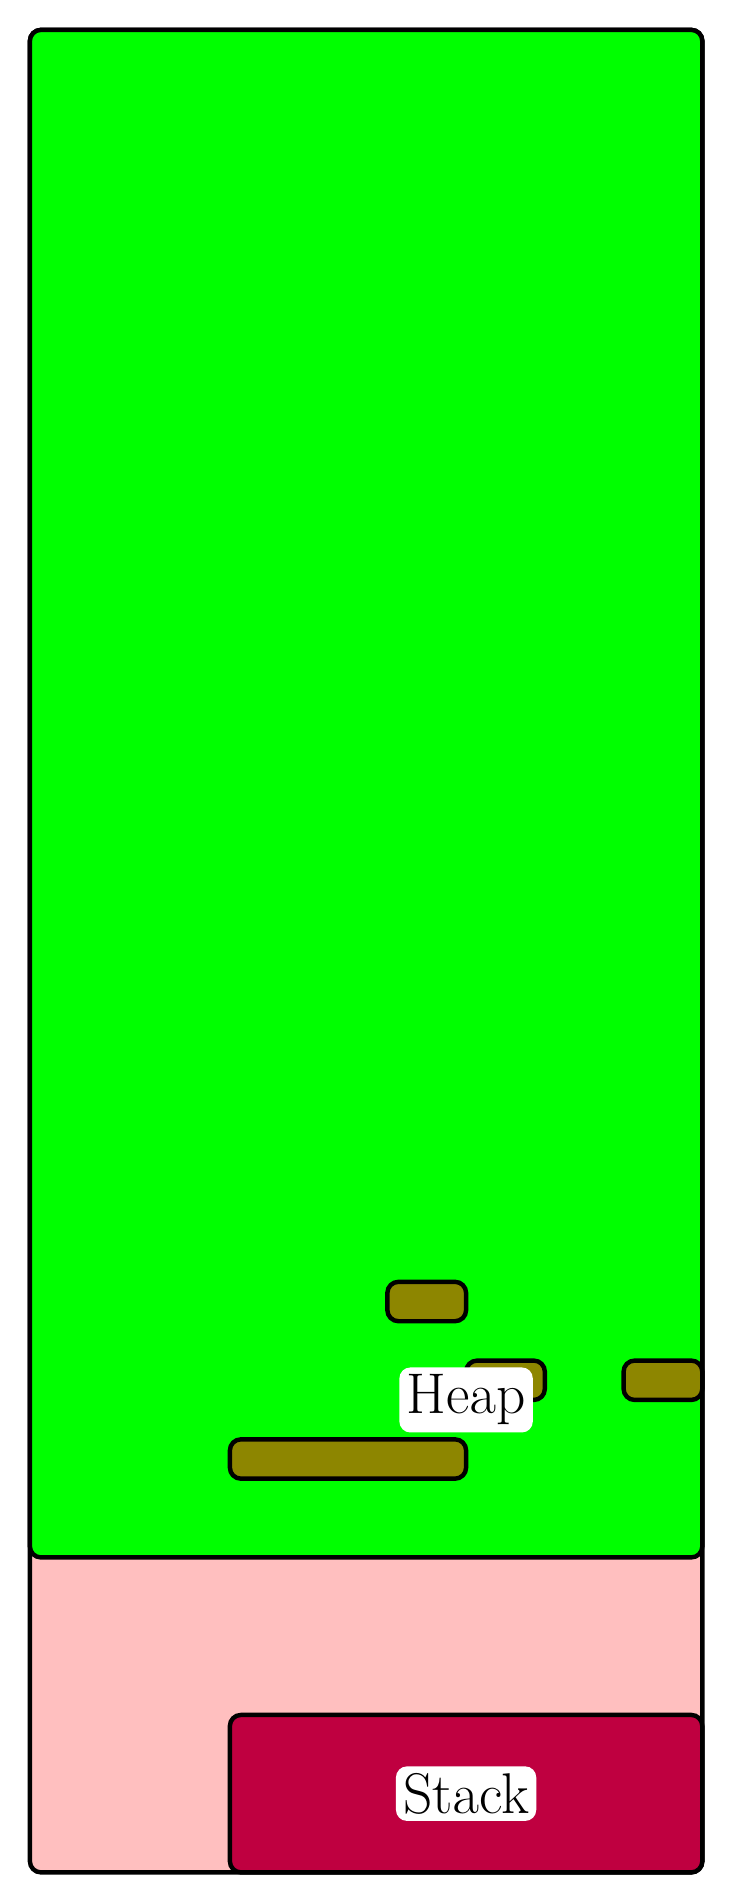
\begin{tikzpicture}[ultra thick, rounded corners]
        \draw [fill=pink] (current page.north west) rectangle (6cm, 2cm);
        \draw [fill=purple] (0cm, 2cm) rectangle (6cm, 4cm) node [align=center, anchor=center, fill=white] at (3cm, 3cm) {\huge{Stack}};
        \draw [fill=green] (current page.north west) rectangle (6cm, 6cm);
        \draw [fill=olive] (2cm, 9cm) rectangle +(1cm, 0.5cm) (3cm, 8cm) rectangle +(1cm, 0.5cm) (5cm, 8cm) rectangle +(1cm, 0.5cm) (0, 7cm) rectangle +(3cm, 0.5cm);
        \draw node [align=center, anchor=center, fill=white] at (3cm, 8cm) {\huge{Heap}};
      \end{tikzpicture}
    \end{column}
  \end{columns}

  \begin{tikzpicture}[callout]
    \draw (4cm, 22em) node [anchor=east] {\shortstack{Find enough space (expensive)}} -> (6.25cm, 5.25cm);
    \draw (4cm, 3em) node [anchor=east] {\shortstack{Increment an address (cheap)}} -> (6.25cm, 1cm);
  \end{tikzpicture}
\end{frame}

\begin{frame}[fragile=singleslide]
  \frametitle{Pointers Vs. References}

  \begin{itemize}
    \item Access lots of data without copying it
    \item Left dangling (\textbf{invalid}) if the referenced object is deallocated
    \begin{itemize}
      \item No way to check for this
      \item Will likely cause a crash if you try to use it
    \end{itemize}
    \item Polymorphism okay
    \item Both compile to similar machine code
    \item Multiple pointers/references can refer to one object
  \end{itemize}

  \begin{columns}
    \begin{column}{6cm}
      \textbf{Pointers:}
      \begin{itemize}
        \item May be invalid (dangling)
        \item Can represent lack of data
        \item Syntax to use and declare
        \item Address can be reassigned
      \end{itemize}
    \end{column}

    \begin{column}{6cm}
      \textbf{References:}
      \begin{itemize}
        \item Always initialized
        \item Points to \textbf{exactly one} address
        \item Less syntax
        \item Easier to deal with objects that shouldn't change
      \end{itemize}
    \end{column}
  \end{columns}
\end{frame}

\begin{frame}[fragile=singleslide]
  \frametitle{Pointers and References}
  \begin{columns}[t]
    \begin{column}{6cm}
      \textbf{Pointers:}
      \cppfile{src/pointers.cpp}
    \end{column}

    \begin{column}{6cm}
      \textbf{References:}
      \cppfile{src/references.cpp}
    \end{column}
  \end{columns}
\end{frame}

\begin{frame}[fragile=singleslide]
  \frametitle{Undefined Behavior}
  \begin{columns}
    \begin{column}{6cm}
      \begin{itemize}
        \item Java fully defines everything
        \item C++ leaves certain edge cases up to the compiler
        \item Many, many ways to invoke
        \item \textbf{Do not rely on UB}
        \begin{itemize}
          \item Best case scenario: Crash
          \item Worst case scenario: No crash
        \end{itemize}
      \end{itemize}
    \end{column}

    \begin{column}{6cm}
      \cppfile{src/ub.cpp}
    \end{column}
  \end{columns}
\end{frame}

\begin{frame}[fragile=singleslide]
  \frametitle{Namespaces}

  \cppfile{src/namespace.cpp}

  
\begin{tikzpicture}[callout]
    \draw (6cm, 22em) node [anchor=west] {\shortstack{Don't do this (or java.util.*)}} -> ([shift={(0em,.25em)}]pic cs:namespace_std);
    \draw (5cm, 19em) node [anchor=west] {\shortstack{Nest them as much as you'd like}} -> ([shift={(0em,.25em)}]pic cs:namespace_nest_a);
    \draw (5cm, 19em) -> ([shift={(0em,.25em)}]pic cs:namespace_nest_b);
    \draw (5cm, 19em) -> ([shift={(0em,.25em)}]pic cs:namespace_nest_c);
    \draw (5cm, 8em) node [anchor=west] {\shortstack{Fully-qualified name}} -> ([shift={(0em,.25em)}]pic cs:namespace_qualified);
    \draw (6cm, 4em) node [anchor=west] {\shortstack{Or bring it into the\\current namespace}} -> ([shift={(0em,.25em)}]pic cs:namespace_using);
  \end{tikzpicture}
\end{frame}

\begin{frame}[fragile=singleslide]
  \frametitle{The Preprocessor}

  \cppfile{src/cpp.cpp}

  
\begin{tikzpicture}[callout]
    \draw (3cm, 25em) node [anchor=west] {\shortstack{Convention: <> for third-party or\\standard library, "" for your code}} -> ([shift={(0em,.25em)}]pic cs:cpp_include);
    \draw (4cm, 21em) node [anchor=west] {\shortstack{Conditional compilation (you can also add\\\#defines through your build process)}} -> ([shift={(0em,.25em)}]pic cs:cpp_define);
    \draw (3cm, 18em) node [anchor=west] {\shortstack{Uncomment these}} -> ([shift={(0em,.25em)}]pic cs:cpp_windows);
    \draw (3cm, 18em) -> ([shift={(0em,.25em)}]pic cs:cpp_mac);
    \draw (4cm, 9em) node [anchor=west] {\shortstack{Contents ignored (not compiled) if on Linux}} -> ([shift={(0em,.25em)}]pic cs:cpp_linux);
    \draw (5cm, 3em) node [anchor=west] {\shortstack{Intentional compiler error}} -> ([shift={(0em,.25em)}]pic cs:cpp_error);
  \end{tikzpicture}
\end{frame}

\begin{frame}[fragile=singleslide]
  \frametitle{Enumerations}

  \cppfile{src/enum.cpp}

  
\begin{tikzpicture}[callout]
    \draw (3cm, 25em) node [anchor=west] {\shortstack{Scoped integers, not objects}} -> ([shift={(0em,.25em)}]pic cs:enum_not_object);
    \draw (3cm, 22em) node [anchor=west] {\shortstack{Trailing comma OK}} -> ([shift={(0em,.25em)}]pic cs:enum_comma);
    \draw (3cm, 17em) node [anchor=west] {\shortstack{OK to assign values}} -> ([shift={(0em,.25em)}]pic cs:enum_value);
    \draw (3cm, 13em) node [anchor=west] {\shortstack{Old-style enums\\(recognize, but avoid)}} -> ([shift={(0em,.25em)}]pic cs:enum_old);
    \draw (5cm, 8em) node [anchor=west] {\shortstack{Scoped enum usage}} -> ([shift={(0em,.25em)}]pic cs:enum_scoped_a);
    \draw (5cm, 8em) -> ([shift={(0em,.25em)}]pic cs:enum_scoped_b);
    \draw (5cm, 5em) node [anchor=west] {\shortstack{Avoid if enum is not contiguous}} -> ([shift={(0em,.25em)}]pic cs:enum_ub);
    \draw (4cm, 3em) node [anchor=west] {\shortstack{Explicitly convert enum to int}} -> ([shift={(0em,.25em)}]pic cs:enum_int);
  \end{tikzpicture}
\end{frame}

\begin{frame}[fragile=singleslide]
  \frametitle{Declaring Classes}

  \cppfile{src/class.cpp}

  
\begin{tikzpicture}[callout]
    \draw (3cm, 17em) node [anchor=west] {\shortstack{REQUIRED for any inheritable class}} -> ([shift={(0em,.25em)}]pic cs:class_virtual_dtor);
    \draw (3cm, 24em) node [anchor=west] {\shortstack{Access modifiers same as in Java}} -> ([shift={(0em,.25em)}]pic cs:class_access_a);
    \draw (4cm, 12em) node [anchor=west] {\shortstack{struct defaults to public\\class defaults to private}} -> ([shift={(0em,.25em)}]pic cs:class_struct);
    \draw (2cm, 14em) node [anchor=west] {\shortstack{Remember the semicolon!}} -> ([shift={(0em,.25em)}]pic cs:class_semicolon);
    \draw (3cm, 22em) node [anchor=west] {\shortstack{Allows method to be overridden}} -> ([shift={(0em,.25em)}]pic cs:class_virtual);
    \draw (9cm, 19em) node [anchor=west] {\shortstack{Technically you can,\\but things get weird}} -> ([shift={(0em,.25em)}]pic cs:class_no_override);
    \draw (2cm, 11em) node [anchor=north] {\shortstack{Abstract method}} -> ([shift={(0em,.25em)}]pic cs:class_abstract);
    \draw (6cm, 4em) node [anchor=north west] {\shortstack{Marks method as an override\\(optional, but recommended)}} -> ([shift={(0em,.25em)}]pic cs:class_override);
    \draw (2cm, 2em) node [anchor=north] {\shortstack{Call parents with class name}} -> ([shift={(0em,.25em)}]pic cs:class_super);
    \draw (7cm, 7em) node [anchor=west] {\shortstack{Inheritance (actually six\\kinds; just use public)}} -> ([shift={(0em,.25em)}]pic cs:class_inheritance);
  \end{tikzpicture}
\end{frame}

\begin{frame}[fragile=singleslide]
  \frametitle{(Con|De)structors, RAII, and the Rule of 3}

  \cppfile{src/raii.cpp}

  
\begin{tikzpicture}[callout]
    \draw (3cm, 27em) node [anchor=west] {\shortstack{Don't write this class\\(STL does it better)}} -> ([shift={(0em,.25em)}]pic cs:raii_dont);
    \draw (5cm, 23em) node [anchor=south] {\shortstack{Member initialization syntax}} -> ([shift={(0em,.25em)}]pic cs:raii_init);
    \draw (8cm, 22em) node [anchor=south west] {\shortstack{Anything else\\(nothing right now)}} -> ([shift={(0em,.25em)}]pic cs:raii_ctor);
    \draw (9cm, 7em) node [anchor=north] {\shortstack{Rule of 3: You need to write one,\\you need to write them all}} -> ([shift={(0em,.25em)}]pic cs:raii_copyctor) node [pos=.5, above, sloped, anchor=north] {Copy constructor};
    \draw (9cm, 7em) -> ([shift={(0em,.25em)}]pic cs:raii_dtor) node [pos=.5, above, sloped, anchor=north] {Destructor};
    \draw (9cm, 7em) -> ([shift={(0em,.25em)}]pic cs:raii_copyeq) node [pos=.5, above, sloped, anchor=north] {Copy assignment};
    \draw (4.5cm, 3em) node [anchor=north] {\shortstack{RAII: Create in ctor, delete in dtor}} -> ([shift={(0em,.25em)}]pic cs:raii_dtor_b);
  \end{tikzpicture}
\end{frame}

\begin{frame}[fragile=singleslide]
  \frametitle{Deleted Functions}

  \cppfile{src/deleted.cpp}

  
\begin{tikzpicture}[callout]
    \draw (8cm, 18em) node [anchor=west] {\shortstack{Forbids this special method\\(compiler error if used)}} -> ([shift={(0em,.25em)}]pic cs:deleted_a);
    \draw (8cm, 18em) -> ([shift={(0em,.25em)}]pic cs:deleted_b);
    \draw (4cm, 14em) node [anchor=west] {\shortstack{Still gotta clean up}} -> ([shift={(0em,.25em)}]pic cs:deleted_cleanup);
    \draw (4cm, 6em) node [anchor=west] {\shortstack{This is how you should use RAII}} -> ([shift={(0em,.25em)}]pic cs:deleted_should);
  \end{tikzpicture}
\end{frame}

\begin{frame}[fragile=singleslide]
  \frametitle{\cppinline{unique_ptr}}

  \cppfile{src/unique.cpp}

  
\begin{tikzpicture}[callout]
    \draw (4cm, 20em) node [anchor=south west] {\shortstack{At most one unique\_ptr\\can manage an address}} -> ([shift={(0em,.25em)}]pic cs:unique_ptr);
    \draw (8cm, 15em) node [anchor=south] {\shortstack{Use make\_unique, not existing\\pointers (else you risk double-deletes)}} -> ([shift={(0em,.25em)}]pic cs:unique_multiple);
    \draw (5cm, 8em) node [anchor=west] {\shortstack{Cleaned up with RAII}} -> ([shift={(0em,.25em)}]pic cs:unique_delete);
  \end{tikzpicture}
\end{frame}

\begin{frame}[fragile=singleslide]
  \frametitle{Casting}

  \cppfile{src/cast.cpp}

  
\begin{tikzpicture}[callout]
    \draw (6cm, 21em) node [anchor=west] {\shortstack{Polymorphism can't be done on values,\\must be pointers or references}} -> ([shift={(0em,.25em)}]pic cs:cast_poly);
    \draw (5cm, 16em) node [anchor=west] {\shortstack{Explicit upcasts rarely necessary}} -> ([shift={(0em,.25em)}]pic cs:cast_upcast_a);
    \draw (5cm, 16em) -> ([shift={(0em,.25em)}]pic cs:cast_upcast_b);
    \draw (6cm, 13em) node [anchor=west] {\shortstack{Runtime type check (slow)}} -> ([shift={(0em,.25em)}]pic cs:cast_dynamic);
    \draw (6cm, 12em) node [anchor=west] {\shortstack{Compile-time type assurance (fast)}} -> ([shift={(0em,.25em)}]pic cs:cast_static);
    \draw (6cm, 9em) node [anchor=west] {\shortstack{Pointer to derived (success)}} -> ([shift={(0em,.25em)}]pic cs:cast_dynamic_pass);
    \draw (6cm, 8em) node [anchor=west] {\shortstack{nullptr (failure, exception if a reference)}} -> ([shift={(0em,.25em)}]pic cs:cast_dynamic_fail);
    \draw (6cm, 6em) node [anchor=west] {\shortstack{Pointer to derived (hopefully success?)}} -> ([shift={(0em,.25em)}]pic cs:cast_static_pass);
    \draw (6cm, 5em) node [anchor=west] {\shortstack{Undefined behavior (hopefully success?)}} -> ([shift={(0em,.25em)}]pic cs:cast_static_fail);
    \draw (3cm, 2em) node [anchor=west] {\shortstack{You fucked up!}} -> ([shift={(0em,.25em)}]pic cs:cast_ub);
  \end{tikzpicture}
\end{frame}

\begin{frame}[fragile=singleslide]
  \frametitle{Concepts}

  \begin{itemize}
    \item Named requirements for a type or function
    \begin{itemize}
      \item Kind of like compile-time interfaces
      \item Usually (but not always) impementing certain methods
    \end{itemize}
    \item Types may be used in templates if they do certain things
    \item Future language revisions will integrate them into the syntax
  \end{itemize}

  \textbf{Examples (simplified):}
  \begin{itemize}
    \item \cppinline{EqualityComparable} $\rightarrow$ provides \cppinline{operator==} for equality test
    \item \cppinline{Container} $\rightarrow$ holds objects and manages their memory (via RAII)
    \item \cppinline{SequenceContainer} $\rightarrow$ \cppinline{Container} whose elements are sequential
    \item \cppinline{FormattedOutputFunction} $\rightarrow$ Function that outputs an object to a \cppinline{std::ostream} (like \cppinline{cout})
  \end{itemize}
\end{frame}

\begin{frame}[fragile=singleslide]
  \frametitle{Templates}

  \cppfile{src/template.cpp}

  
\begin{tikzpicture}[callout]
    \draw (3cm, 25em) node [anchor=south west] {\shortstack{Standard library uses\\LOTS of templates}} -> ([shift={(0em,.25em)}]pic cs:template_stl);
    \draw (7cm, 22em) node [anchor=west] {\shortstack{Almost anything can be templated}} -> ([shift={(0em,.25em)}]pic cs:template_class) node [pos=.5, above, sloped, anchor=south] {classes};
    \draw (7cm, 22em) -> ([shift={(0em,.25em)}]pic cs:template_typedef) node [pos=.5, above, sloped, anchor=north] {typedefs};
    \draw (7cm, 22em) -> ([shift={(0em,.25em)}]pic cs:template_function) node [pos=.5, above, sloped, anchor=north] {(member )?functions};
    \draw (3cm, 11em) node [anchor=west] {\shortstack{For types that depend on template parameters inside templates}} -> ([shift={(0em,.25em)}]pic cs:template_depend);
    \draw (6cm, 7em) node [anchor=west] {\shortstack{Three different classes\\and chunks of code}} -> ([shift={(0em,.25em)}]pic cs:template_diff_a);
    \draw (6cm, 7em) -> ([shift={(0em,.25em)}]pic cs:template_diff_b);
    \draw (6cm, 7em) -> ([shift={(0em,.25em)}]pic cs:template_diff_c);
    \draw (3cm, 4.5em) node [anchor=west] {\shortstack{Function type parameters can be deduced}} -> ([shift={(0em,.25em)}]pic cs:template_function_deduce);
    \draw (3cm, 3em) node [anchor=west] {\shortstack{Error: No way to print a Dummy}} -> ([shift={(0em,.25em)}]pic cs:template_no_print);
  \end{tikzpicture}
\end{frame}

\begin{frame}[fragile=singleslide]
  \frametitle{\cppinline{assert}/\cppinline{static_assert}}

  \cppfile{src/assert.cpp}

  
\begin{tikzpicture}[callout]
    \draw (3cm, 24em) node [anchor=west] {\shortstack{Standard "debug mode" \#define}} -> ([shift={(0em,.25em)}]pic cs:assert_ndebug);
    \draw (4cm, 8em) node [anchor=west] {\shortstack{Only run in debug builds (don't\\do side effects or error checking)}} -> ([shift={(0em,.25em)}]pic cs:assert_use);
    \draw (6cm, 4em) node [anchor=west] {\shortstack{OK}} -> ([shift={(0em,.25em)}]pic cs:assert_ok_a);
    \draw (6cm, 4em) -> ([shift={(0em,.25em)}]pic cs:assert_ok_b);
    \draw (5cm, 2em) node [anchor=west] {\shortstack{Compiler error, as desired}} -> ([shift={(0em,.25em)}]pic cs:assert_error);
  \end{tikzpicture}
\end{frame}

\begin{frame}[fragile=singleslide]
  \frametitle{\cppinline{const}}

  \cppfile{src/const.cpp}

  
\begin{tikzpicture}[callout]
    \draw (9cm, 21em) node [anchor=west] {\shortstack{No side effects\\(aka state changes)}} -> ([shift={(0em,.25em)}]pic cs:const_nochange);
    \draw (9cm, 18em) node [anchor=west] {\shortstack{Immutable reference\\(no state changes)}} -> ([shift={(0em,.25em)}]pic cs:const_ref);
    \draw (9cm, 15em) node [anchor=west] {\shortstack{Mutable reference\\(state changes possible)}} -> ([shift={(0em,.25em)}]pic cs:const_nonconst_ref);
    \draw (8cm, 12em) node [anchor=west] {\shortstack{Side effects}} -> ([shift={(0em,.25em)}]pic cs:const_nonconst);
    \draw (4cm, 11em) node [anchor=west] {\shortstack{Bypassing const through\\tricks is usually UB}} -> ([shift={(0em,.25em)}]pic cs:const_ub);
    \draw (8cm, 3em) node [anchor=west] {\shortstack{const forbids state changes\\(thus won't compile)}} -> ([shift={(0em,.25em)}]pic cs:const_no_cat);
    \draw (6cm, 7em) node [anchor=west] {\shortstack{One name, two overloads\\(chosen by compiler)}} -> ([shift={(0em,.25em)}]pic cs:const_overload_a);
    \draw (6cm, 7em) -> ([shift={(0em,.25em)}]pic cs:const_overload_b);
  \end{tikzpicture}
\end{frame}

\begin{frame}[fragile=singleslide]
  \frametitle{Operator Overloading}

  \cppfile{src/operator.cpp}

  
\begin{tikzpicture}[callout]
    \draw (4cm, 25em) node [anchor=west] {\shortstack{cout is a global std::ostream}} -> ([shift={(0em,.25em)}]pic cs:operator_cout);
    \draw (6.5cm, 16em) node [anchor=west] {\shortstack{Make a type printable (technically doesn't\\fully meet FormattedOutputFunction)}} -> ([shift={(0em,.25em)}]pic cs:operator_ostream);
    \draw (7.5cm, 21em) node [anchor=west] {\shortstack{overloads should be sensible}} -> ([shift={(0em,.25em)}]pic cs:operator_sensible);
    \draw (7cm, 12em) node [anchor=west] {\shortstack{Meets EqualityComparable}} -> ([shift={(0em,.25em)}]pic cs:operator_eq);
  \end{tikzpicture}
\end{frame}

\begin{frame}[fragile=singleslide]
  \frametitle{Data Structures}
  \begin{itemize}
    \item Remember to \cppinline{#include <class_name>}!
    \item Prefer \cppinline{std::array<SomeType, Length>} to \cppinline{SomeType[Length]}
    \item Java describes behavior with interfaces, C++ with concepts
  \end{itemize}
  \begin{columns}
    \begin{column}{6cm}
      \begin{itemize}
        \item \cppinline{vector<T>}
        \item \cppinline{deque<T>}
        \item \cppinline{list<T>}
        \item \cppinline{set<T>}
        \item \cppinline{map<T, U>}
        \item \cppinline{unordered_set<T>}
        \item \cppinline{unordered_map<T, U>}
        \item \cppinline{stack<T>}
        \item \cppinline{priority_queue<T>}
      \end{itemize}
    \end{column}

    \begin{column}{6cm}
      \begin{itemize}
        \item \javainline{ArrayList<T>}
        \item \javainline{ArrayQueue<T>}
        \item \javainline{LinkedList<T>}
        \item \javainline{TreeSet<T>}
        \item \javainline{TreeMap<T, U>}
        \item \javainline{HashSet<T>}
        \item \javainline{HashMap<T, U>}
        \item \javainline{Stack<T>}
        \item \javainline{PriorityQueue<T>}
      \end{itemize}
    \end{column}
  \end{columns}
\end{frame}

\begin{frame}[fragile=singleslide]
  \frametitle{String to numbers and back}

  \cppfile{src/stoi.cpp}

  
\begin{tikzpicture}[callout]
    \draw (4cm, 17em) node [anchor=west] {\shortstack{sto(i|u?ll?|f|l?d) is available, too}} -> ([shift={(0em,.25em)}]pic cs:stoi_stoi);
    \draw (4cm, 12em) node [anchor=west] {\shortstack{Or std::to\_wstring}} -> ([shift={(0em,.25em)}]pic cs:stoi_wstring);
    \draw (4cm, 10em) node [anchor=west] {\shortstack{a == 42}} -> ([shift={(0em,.25em)}]pic cs:stoi_a);
    \draw (7cm, 8em) node [anchor=west] {\shortstack{b == 9\\(strips whitespace, reads as base-16)}} -> ([shift={(0em,.25em)}]pic cs:stoi_b);
    \draw (8cm, 3em) node [anchor=north] {\shortstack{c == 2\\first\_nonnumeric\_char\_index == 2}} -> ([shift={(0em,.25em)}]pic cs:stoi_c);
    \draw (4cm, 3em) node [anchor=west] {\shortstack{"12"}} -> ([shift={(0em,.25em)}]pic cs:stoi_back);
  \end{tikzpicture}
\end{frame}

\begin{frame}[fragile=singleslide]
  \frametitle{Regexes}

  \cppfile{src/regex.cpp}

  
\begin{tikzpicture}[callout]
    \draw (4cm, 23em) node [anchor=west] {\shortstack{search for finding substrings,\\match for matching whole strings}} -> ([shift={(0em,.25em)}]pic cs:regex_match);
    \draw (6cm, 17em) node [anchor=south] {\shortstack{ECMAScript syntax by\\default, but others available}} -> ([shift={(0em,.25em)}]pic cs:regex_syntax);
    \draw (8cm, 16em) node [anchor=west] {\shortstack{Case insensitive flag}} -> ([shift={(0em,.25em)}]pic cs:regex_flags);
    \draw (8cm, 11em) node [anchor=west] {\shortstack{Returns true if a\\match was found}} -> ([shift={(0em,.25em)}]pic cs:regex_search);
    \draw (7cm, 8em) node [anchor=west] {\shortstack{Class to store actual match\\results and positions}} -> ([shift={(0em,.25em)}]pic cs:regex_smatch_a);
    \draw (7cm, 8em) -> ([shift={(0em,.25em)}]pic cs:regex_smatch_b);
    \draw (7cm, 2em) node [anchor=west] {\shortstack{Actually accessing matches}} -> ([shift={(0em,.25em)}]pic cs:regex_access_match);
  \end{tikzpicture}
\end{frame}

\begin{frame}[fragile=singleslide]
  \frametitle{Custom Map Keys}

  \cppfile{src/map.cpp}

  
\begin{tikzpicture}[callout]
    \draw (6cm, 23em) node [anchor=west] {\shortstack{For use in ordered (tree-based)\\associative containers}} -> ([shift={(0em,.25em)}]pic cs:map_lt);
    \draw (5cm, 13em) node [anchor=west] {\shortstack{For use in unordered (hash-based)\\associative containers}} -> ([shift={(0em,.25em)}]pic cs:map_eq);
    \draw (5cm, 13em) -> ([shift={(0em,.25em)}]pic cs:map_hash);
    \draw (8cm, 9em) node [anchor=west] {\shortstack{Required for std::hash\\specializations}} -> ([shift={(0em,.25em)}]pic cs:map_arg);
    \draw (8cm, 9em) -> ([shift={(0em,.25em)}]pic cs:map_result);
    \draw (8cm, 9em) -> ([shift={(0em,.25em)}]pic cs:map_func);

  \end{tikzpicture}
\end{frame}

\begin{frame}[fragile=singleslide]
  \frametitle{Random Numbers}

  \cppfile{src/random.cpp}

  
\begin{tikzpicture}[callout]
    \draw (4cm, 12em) node [anchor=west] {\shortstack{OS/hardware's source of randomness}} -> ([shift={(0em,.25em)}]pic cs:random_device);
    \draw (5cm, 10em) node [anchor=west] {\shortstack{Initialize a PRNG with a seed}} -> ([shift={(0em,.25em)}]pic cs:random_init);
    \draw (6cm, 6em) node [anchor=north west] {\shortstack{LOTS of distributions available\\(did you take AMS 310 yet?)}} -> ([shift={(0em,.25em)}]pic cs:random_many);
    \draw (3cm, 1em) node [anchor=north] {\shortstack{Or use any UniformRandomNumberGenerator\\(including random\_device, but it's slow)}} -> ([shift={(0em,.25em)}]pic cs:random_concept);
  \end{tikzpicture}
\end{frame}

\begin{frame}[fragile=singleslide]
  \frametitle{Formatted Output and String Concatenation}

  \cppfile{src/formatted.cpp}

  
\begin{tikzpicture}[callout]
    \draw (4cm, 16em) node [anchor=west] {\shortstack{Changes how floats are printed out\\(many modifiers exist)}} -> ([shift={(0em,.25em)}]pic cs:formatted_modifier);
    \draw (4cm, 12em) node [anchor=west] {\shortstack{std::ostream that writes to a string}} -> ([shift={(0em,.25em)}]pic cs:formatted_stringstream);
    \draw (5cm, 2em) node [anchor=north west] {\shortstack{Use stringstream for nontrivial formats (a la printf)\\Use string::operator+ for concatenation\\Use sto(i|u?ll?|f|l?d) for number conversions}} -> ([shift={(0em,.25em)}]pic cs:formatted_str);
  \end{tikzpicture}
\end{frame}

\begin{frame}[fragile=singleslide]
  \frametitle{Iterators}

  \cppfile{src/iterator.cpp}

  
\begin{tikzpicture}[callout]
    \draw (3cm, 13em) node [anchor=west] {\shortstack{Deduce the type\\(for when its name is long)}} -> ([shift={(0em,.25em)}]pic cs:iterator_auto);
    \draw (8cm, 8em) node [anchor=west] {\shortstack{Probably an ordinary pointer\\(but that's not your concern)}} -> ([shift={(0em,.25em)}]pic cs:iterator_ptr);
    \draw (5cm, 5em) node [anchor=west] {\shortstack{Iteratee must provide\\begin and end methods}} -> ([shift={(0em,.25em)}]pic cs:iterator_begin);
    \draw (3cm, 3em) node [anchor=north west] {\shortstack{Remember to iterate by reference\\(and const if not changing the data)}} -> ([shift={(0em,.25em)}]pic cs:iterator_ref);
  \end{tikzpicture}
\end{frame}

\begin{frame}[fragile=singleslide]
  \frametitle{Anonymous functions and \cppinline{<algorithm>}}

  \cppfile{src/lambda.cpp}

  
\begin{tikzpicture}[callout]
    \draw (7cm, 18em) node [anchor=west] {\shortstack{Lambda return type\\(omit to deduce)}} -> ([shift={(0em,.25em)}]pic cs:lambda_return);
    \draw (7cm, 14em) node [anchor=west] {\shortstack{Omit parens if there are no arguments}} -> ([shift={(0em,.25em)}]pic cs:lambda_parens);
    \draw (7cm, 9em) node [anchor=south] {\shortstack{Capture ints by reference\\(omit \& for value capture)}} -> ([shift={(0em,.25em)}]pic cs:lambda_capture);
    \draw (3.5cm, 7em) node [anchor=south] {\shortstack{Run over entire ints array}} -> ([shift={(0em,.25em)}]pic cs:lambda_begin);
    \draw (3.5cm, 7em) -> ([shift={(0em,.25em)}]pic cs:lambda_end);
    \draw (6cm, 3em) node [anchor=west] {\shortstack{Output iterator is same as input\\(so it operates in-place)}} -> ([shift={(0em,.25em)}]pic cs:lambda_inplace);
  \end{tikzpicture}
\end{frame}

\begin{frame}[fragile=singleslide]
  \frametitle{Time}

  \cppfile{src/time.cpp}

  
\begin{tikzpicture}[callout]
    \draw (4cm, 23em) node [anchor=west] {\shortstack{Threading is a whole new\\can of worms (let's not open it)}} -> ([shift={(0em,.25em)}]pic cs:time_thread);
    \draw (6cm, 20em) node [anchor=west] {\shortstack{Convert between units of time}} -> ([shift={(0em,.25em)}]pic cs:time_cast);
    \draw (7cm, 17em) node [anchor=west] {\shortstack{Really a typedef for a generic duration\\(you can define your own units)}} -> ([shift={(0em,.25em)}]pic cs:time_duration);
    \draw (6cm, 14em) node [anchor=west] {\shortstack{Several types of clocks exist}} -> ([shift={(0em,.25em)}]pic cs:time_clock);
    \draw (7cm, 11em) node [anchor=west] {\shortstack{Durations accept integers (but\\you can define float typedefs)}} -> ([shift={(0em,.25em)}]pic cs:time_ctor);
    \draw (5cm, 6em) node [anchor=west] {\shortstack{Your game's timer can\\(and should) use only std::chrono}} -> ([shift={(0em,.25em)}]pic cs:time_loop);
  \end{tikzpicture}
\end{frame}

\begin{frame}[fragile=singleslide]
  \frametitle{Next Week}
  \begin{itemize}
    \item Compiling and linking code
    \item Dealing with multiple files
    \item Using Visual Studio
    \item Overview of popular C++ tools
    \item Building and using a library
  \end{itemize}
\end{frame}

\begin{frame}[fragile=singleslide]
  \frametitle{Thank You!}
  \begin{itemize}
    \item Find these slides on GitHub
  \end{itemize}
\end{frame}

\end{document}